\documentclass[uplatex,dvipdfmx]{jsarticle}

\input{"preamble.tex"}

\title{Phonons in a condensed boson gas}
\author{ガオゾウ}

\begin{document}
\maketitle
\section{概要}
C.KittelのQuantum theory of solidsの第二章中のPHONONS IN A CONDENSED BOSON GASに関するまとめです。

\section{本題}
弱く相互作用するボゾンガスを考えます。
\begin{figure}[htbp]
	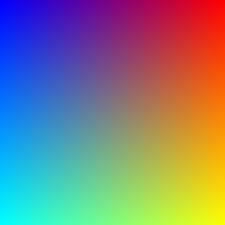
\includegraphics[width=5cm]{sample.jpg}
\end{figure}

この系のハミルトニアンは次のように与えられるものとします。
\end{document}